\section{General Implementation}
Before entering specifics of the Lotka-Volterra and Type 1 Diabetes systems, it is best to gain a general understanding of how to tune each aspect of the UKF algorithm. We will do this by separating out discussion of the Joint and Dual algorithms. However, it is first necessary to discuss parameter values that are common to both.

\subsection{Common Parameters}
As discussed earlier, the basis of the UKF, the Unscented Transformation, involves the creation of a vector of sigma points. In the creation of the Sigma Point vector in the UKF, two parameters determine the distance between these points, namely $\alpha$ and $\kappa$. In particular, both are incorporated in calculating the scaling parameter $\lambda$ through:
$$\lambda = \alpha^2 (L + \kappa) - L$$
where $L$ is the number of states.\\
\\

From previous work (Van Mere), we know $\alpha$ is set to a value between 1e-4 and 1. Intuitively, the larger the value of $\alpha$, the larger the spread of sigma points. In our work, we have used values closer to 1e-4, as will be noted in the Predator Prey and T1D sections. $\kappa$, similarly, is a scaling parameter set to 0 or $3 - L$ (Van Mere). From our work we have found a value of 0 to work best. However, $\alpha$ and $\kappa$ did not appear to have drastic impacts on our results, and we have found that spreading of sigma points is better controlled by covariance matrices than the $\alpha$ and $\kappa$ parameters. The final parameter common to both the Dual and Joint is $\beta$, which is used to capture prior knowledge one has about the latent states. For an assumed Gaussian distribution, $\beta$ equal to 2 has been used (Van Mere).\\
\\
In addition to these three parameters, the tuning of noise and initial state covariance matrices is necessary in both cases. Process noise is often difficult to calculate due to unknown states. We have found different optimal values for process noise in the Dual and Joint UKFs, which will be discussed in their respective sections moving forward. Measurement Noise needs to be similarly tuned. If one has explicit knowledge of how the data they are working with has been gathered, this can inform the decision of measurement noise covariance. However, since this is unavailable in the context of both Predator-Prey and T1D, they have been determined in an ad-hoc fashion. We have found that values on the same order of magnitude as the data itself work best. Moreover, measurement of observable populations are assumed to be independent in this context, meaning that no covariance is assigned between them, but rather a diagonal matrix is used to represent variance for measurement noise. Let us now go through the setup of each type of UKF individually to consider and compare their differences.


\subsection{Joint UKF}

In the Joint UKF, since states and parameters are estimated simultaneously in the same vector, there are three tunable matrices that must be initialized, the process noise $Q$, the measurement noise $R$, and the initial covariance matrix of states and parameters $P_0$. 

\subsubsection{Process Noise $Q$}
In the Joint UKF, noise related to the states and noise related to the parameters is not separated. Thus, one must be particularly careful about how they set up this matrix. In our experience, these values will need to be tuned based on the specific model set up. However, two aspects are consistently important across models. Firstly, assigning too high of variance values to the parameter noise can have severe consequences on the performance of the filter, so one must be sure to tune these especially closely. Secondly, diagonal matrices seem to work best, with 0's in the off-diagonal spots. \\
\\
Lastly, one must make sure that the noise assigned to states is not too large. In our experimentation, assignment of large values to the state variances caused parameters to struggle to move from there original values. This can be explained intuitively by thinking about the meaning of process noise: Telling the algorithm that there is a lot of process noise causes the algorithm to expect much randomness in the data. As a result, when it sees randomness, it is less inclined to move parameters around since these deviations from the standard projection are attributed to noise rather than a need to shift around parameters. This problem, however, is solved once we move to the Dual UKF.

\subsubsection{Measurement Noise $R$}
The measurement noise determines how closely one should trust the observable values being inputted into the model. Large variance values will result in less trust in the observable, and thus a smaller correction through the Kalman Gain, whereas small values will have the opposite effect. This parameter is one which is not very much dependent on the type of UKF algorithm being used. Since the same observables are used whether one chooses a joint or dual UKF, in our work $R$ was set to the same matrix for both algorithms in order to ensure consistency. 

\subsubsection{Initial Covariance $P_0$}
The Joint UKF's combination of states and parameters into a single vector provides us with a great benefit when working with the covariance matrix. Namely, we are able to have covariances between states and parameters. Intuitively, this is a big advantage. For example, consider $\beta$, the predator growth rate in the Predator-Prey model. This parameter should be directly related to what the predator population values are, meaning that there is covariance between the two. The same idea extends to the T1D set up as well.\\
\\
However, we must be sure to not allow for parameter covariances to overwhelm the algorithm. By this, we mean that a change in one parameter must \emph{influence} changes in others but not be the main determinant. Thus, covariances between the parameters have been set to relatively small values, dependent on the model. Next, we will need to identify variances for states and parameters. These variances are critical as they will play a role both in the Joint, as well as Dual, UKF's.\\
\\
Parameter variances in particular are crucial to the amount of movement a parameter will go through over the course of a UKF run. By assigning a larger variance to a parameter, the user is encouraging the paramter to search, through the Sigma Point vectors, more of the parameter space that surrounds its starting point, and vice versa with smaller variances. Thus, in our experience it has been worth the time to fine tune these values.


\subsubsection{Troubleshooting the Joint UKF}
The two most critical features that led to success of the Joint UKF were allowance of covariance between states and parameters, as well as ensuring that the process noise variance values were sufficiently low. Without \emph{both} of these features, the results we achieved were not satisfactory. Thus, these should be the first two places one looks to when tuning the joint UKF.




\subsection{Dual UKF}
We now consider the manner in which the Dual UKF is implemented generally, as well as its differences as compared to the Joint scenario. The Dual UKF has the following six tunable matrices: the process noise matrices $Q_x$ and $Q_{param}$, the measurement noise matrices $R_x$ and $R_{param}$, and the initial covariance matrices $P_{x_0}$ and $P_{param_0}$. Since the same measurements are used for both the state and parameter estimates, we should have that $R_{param} = R_x$.\\

\subsubsection{Process Covariances}
By separating process noise between the states and parameters, we now have much more control over the setup. Beginning with the state process noise, we often need to determine it in an ad hoc fashion due to unknown state values. In the case of known states, as is the case of Predator-Prey, this can in fact be determined analytically. It is important to note that even if it can be determined analytically here, this approach \emph{did not} prove successful when applied to the Joint UKF, due to the issues of high process noise being assigned to populations as discussed earlier. Next, consider the parameter process noise $Q_{param}$. According to previous literature, %INSERT GOVE CITATION HERE%
it is best to set it to $((1/\lambda) - 1) * P_{param_0}$ where $\lambda$ is between 0 and 1. However, larger values of $\lambda$ produce more stable filters, so we have used a value of 0.99, meaning that we had
$$ Q_{param} = .01 * P_{param_0} $$
 Next, we need to discuss the initial covariance matrices of the states and parameters.

\subsubsection{Initial State and Parameter Covariances}
Instead of a single covariance matrix, as is in the Joint, the Dual has two covariance matrices, one for the states, $P_{x_0}$,  and one for the parameters, $P_{params_0}$. This means that we now need to tune both $P_{x_0}$ and $P_{params_0}$. Let's begin with $P_{x_0}$. This matrix controls the amount of space that the algorithm searches in through its impact on the range of sigma points that are chosen. Thus, if you want to search more of the available space, $P_{x_0}$ should be higher, and if you are more confident in the space you begin in, then it should be lower.
\\
$P_{params_0}$ has proved to be one of, if not the, most important parameter in the Dual UKF. This variable directly determines the amount of parameter space that you will search during the UKF process. Higher values for a parameter variance will search more space and thus can result in larger deviations from the initial values, while smaller variances result in parameter searching more closely to the baseline. When choosing a variance for a particular parameter, it is important to understand that whether a variance is "large" or "small" is dependent on the range that value can take on. For example, if a parameter's baseline value is 5000, a variance of 1 is small, whereas if the baseline value is 10e-3, 1 is quite large. Thus, assigning variances must be done on a parameter by parameter basis. 


\subsection{A General Note on Parameter Variances}
The variance assigned to a parameter value has proven to be very influential on a parameter's final value. Thus, for each parameter in a given system, a sufficient deal of thought must be given to determining a variance value. When doing so, the following three questions are key to consider:
\begin{enumerate}
    \item What is the allowable range of the parameter from a biological or physical standpoint?
    \item How sensitive is the parameter?
    \item How confident is one in the initial parameter guess?
\end{enumerate}
Through use of these questions as guiding principles as well as additional trial and error, one can expect to determine reasonable parameter variances for their given situation.


\section{Implementation on Predator-Prey}
We will now discuss the process of using the Unscented Kalman filter to estimate both states and parameters in the context of the Lotka-Volterra Predatory-Prey system. Both Joint and Dual UKF's were used to fit the model. In the following sections, we will describe the steps for both methods and compare them. First let us establish what our various sets of variables of the UKF represent in the context of Predator-Prey.

\subsection{Model Set Up}
The Lotka-Volterra system consists of prey (Hare) and predator (Lynx) populations as described by the state vector, $x_k$ below \\
$$x_k = [H, L]$$
as well as the parameter set
$$ \theta = [\alpha, \beta, \gamma, \delta] $$
Thus, when we refer to \emph{states} in this section we are referencing the populations, while \emph{parameters} is used to discuss $\theta$. \\
\\
In the case of this system, the observables are the same as the states, which makes the observable vector, $y_k$
$$y_k = [H, L]$$
We will first consider the aspects of the UKF that are common to both the Dual and Joint, and following that, we will discuss the differences.

\subsection{Common Parameters}
Beginning with the common parameter $\alpha$, in our work we have used 1e-3 both for the dual and joint. Secondly, as stated earlier, a $\kappa$ value of 0 has been used and $\beta$ equal to 2. Measurement noise, as stated earlier, should also be consistent across the Joint and Dual due to the same set of measurements being used. Through ad hoc means we have determined
$$R = \begin{bmatrix}
30 & 0\\0 & 15\end{bmatrix}$$
to work best.
Let us now go through the setup of each type of UKF individually to consider and compare their differences.

\subsection{Joint UKF}

In the Joint UKF, we treat the states and parameters as one long state vector, and making our total state vector in this case
$$x_k = [H, L, \alpha, \gamma, \beta, \delta]$$
Our observable vector remains the same, as shown
$$y_k = [H, L]$$
This makes our state space model in this case:
$$x_k = \begin{bmatrix}
H\\
L\\
\alpha\\
\gamma\\
\beta\\
\delta
\end{bmatrix} = \begin{bmatrix}
f_H(H,L,\alpha, \gamma, \beta, \delta)\\
f_L(H,L,\alpha, \gamma, \beta, \delta)\\
\alpha\\
\gamma\\
\beta\\
\delta\\
\end{bmatrix} + \begin{bmatrix}
q_H\\
q_L\\
q_{\alpha}\\
q_{\gamma}\\
q_{\beta}\\
q_{\delta}
\end{bmatrix}$$
$$y_k = \begin{bmatrix}
y_1\\
y_2\\
\end{bmatrix} = 
\begin{bmatrix}
1 & 0 & 0 & 0 & 0 & 0\\
0 & 1 & 0 & 0 & 0 & 0\\
\end{bmatrix}
\begin{bmatrix}
H\\
L\\
\alpha\\
\gamma\\
\beta\\
\delta
\end{bmatrix}+
\begin{bmatrix}
r_1\\
r_2\\
\end{bmatrix}$$
Where $f_H$ and $f_L$ are the solutions to the Lotka-Volterra ODE model, which will be approximated in our code, $q_H$, $q_L$, $q_{alpha}$, $q_{gamma}$, $q_{beta}$, $q_{delta}$ represent the added process noise, $r_1$ and $r_2$ represent the added measurement noise, and $y_1$ and $y_2$ represent the two observables, which in this case are the same as our states $H$ and $L$. Note that in this case, the observables equation, is a linear equation, however that will not always be the case. 

\subsubsection{Process Noise $Q$}
On the predator prey model, keeping the values of $Q$ low has proved crucial. In our experience, we have settled on a diagonal matrix with 10e-5 across the diagonal as the process noise covariance, as in the matrix

$$Q = \begin{bmatrix}
10e-5 & 0 & 0 & 0 & 0 & 0\\
0 & 10e-5 & 0 & 0 & 0 & 0\\
0 & 0 & 10e-5 & 0 & 0 & 0\\
0 & 0 & 0 & 10e-5 & 0 & 0\\
0 & 0 & 0 & 0  & 10e-5 & 0\\
0 & 0 & 0 & 0 & 0 & 10e-5\end{bmatrix}$$

Interestingly, assignment of large values to the state variances caused parameters to struggle to move from there original values, as stated is possible earlier. 

\subsubsection{Initial Covariance $P_0$}
In order to allow for some but not an overwhelming amount of covariance between parameters, these covariances have been set to 0.01. Next, we need to identify variances for the two populations as well as our 4 parameters. For the prey and predator populations, variances of 20 and 15 have been found to work best. Next, $\alpha$ is assigned variance 0.5, $\gamma$ variance 0.3, $\beta$ variance 0.02 and $\delta$ variance 0.02. Note that $\beta$ has proven to be extremely sensitive in this algorithm, particularly in the context of the Joint UKF, and thus is the one parameter with a different variance when turning later on to the Dual. These variances are then all combined together into a single matrix to create
$$P_{0} = \begin{bmatrix}
20 & .01 & .01 & .01 & .01 & .01\\
.01 & 15 & .01 & .01 & .01 & .01\\
.01 & .01 & .5 & .01 & .01 & .01\\
.01 & .01 & .01 & 0.3 & .01 & .01\\
.01 & .01 & .01 & .01  & .02 & .01\\
.01 & .01 & .01 & .01 & .01 & .02\end{bmatrix}$$


\subsubsection{Joint UKF Results}
When assessing the performance of a UKF algorithm, there are multiple characteristics to keep in mind. First, we are interested in the quality of the state estimation. Secondly, we would like to assess the quality of the parameter estimation. Beginning with state estimation, we plot the raw Lotka-Volterra data on top of our state estimates in Figure 1 to get a visual understanding of our performance, and then can calculate mean squared error (MSE) values to assess quality as well, as shown in Table 1. For MSE, we only consider the second half of the data set (values 45 to 91), in order to allow for sufficient time for the algorithm to learn before being judged.\\ 


\begin{figure}[H]
    \centering
    \includegraphics[width=15cm]{Kalman Filter Images/Joint_StateEstimation.jpg}
    \caption{State estimation of Hare and Lynx data using Joint UKF. The estimates produced by each step of the filter are plotted on top of raw data.}
\end{figure}


%INSERT CHART OF MSE
As is evident visually, the Joint UKF is successful at performing state estimation. Although we do miss a few of the peaks in the dataset, the overall performance is very much satisfactory. Next, we would like to understand the amount of parameter movement occurring during the algorithm run. To do so, we plot values of the four parameters at each iteration, as well as a solid line signifying the starting point:\\

\begin{figure}[H]
    \centering
    \includegraphics[width=15cm]{Kalman Filter Images/Joint_ParamatersOverTime.jpg}
    \caption{Movement of Lotka-Volterra parameters as more iterations of Joint UKF are performed.}
\end{figure}


It is evident that there are varying amounts of parameter movement, which is dependent on the quality of the starting guess. Additionally, parameters $\beta$ and $\delta$ appear to follow an oscillatory behavior. This is likely due to the underlying time dependence in these parameters. As discussed in \textbf{Model Setup}, the parameters are assumed to be constant values. However, since the size of the peaks, troughs, and time between them is not consistent in this dataset, it is likely that the parameters are not in fact consistent, due to outside factors not included in this model. Thus, is it is likely that these parameters are oscillating in response to this phenomenon.\\
\\

Moreover, we can see, particularly for $\alpha$ and $\gamma$, that the parameters are beginning to converge towards the latter portion of the runtime. The final assessment of the algorithm's success is to understand the quality of the final parameter estimates, which will be done in the \textbf{Dual UKF} portion of the Lotka-Volterra Section.


\subsection{Dual UKF}
We now consider the manner in which the Dual UKF was implemented for the Predator Prey model. Since the Dual UKF runs two filters simultaneously, we must set up two different state space models, one for the states and one for the parameters. For the states, we have:
$$x_k = \begin{bmatrix}
H\\
L\\
\end{bmatrix} = \begin{bmatrix}
f_H(H,L)\\
f_L(H,L)\\
\end{bmatrix} + \begin{bmatrix}
q_H\\
q_L\\
\end{bmatrix}$$
$$y_k = \begin{bmatrix}
y_1\\
y_2\\
\end{bmatrix} = 
\begin{bmatrix}
1 & 0\\
0 & 1\\
\end{bmatrix}
\begin{bmatrix}
H\\
L\\
\end{bmatrix}+
\begin{bmatrix}
r_1\\
r_2\\
\end{bmatrix}$$

As in the Joint, $f_H$ and $f_L$ are the solutions to the Lotka-Volterra ODE model, which will be approximated in our code, $q_H$ and $q_L$ represent the added process noise, $r_1$ and $r_2$ represent the added measurement noise, and $y_1$ and $y_2$ represent the two observables, which in this case are the same as our states $H$ and $L$.\\
The state space model for the parameters is
$$x_k = \begin{bmatrix}
\alpha\\
\gamma\\
\beta\\
\delta
\end{bmatrix} = \begin{bmatrix}
\alpha\\
\gamma\\
\beta\\
\delta\\
\end{bmatrix} + \begin{bmatrix}
q_{\alpha}\\
q_{\gamma}\\
q_{\beta}\\
q_{\delta}
\end{bmatrix}$$
$$y_k = \begin{bmatrix}
y_1\\
y_2\\
\end{bmatrix} = 
\begin{bmatrix}
f_{H}'(\alpha, \gamma, \beta,\delta)\\
f_{L}'(\alpha, \gamma, \beta,\delta)
\end{bmatrix}+
\begin{bmatrix}
r_1\\
r_2\\
\end{bmatrix}$$
We define $f_H'$ to be some function of $\alpha, \gamma, \beta$ and $\delta$ such that $f_H' = H$ and $f_L'$ to be  some function of $\alpha, \gamma, \beta$ and $\delta$ such that $f_L' = L$. Notice that there is no transition function for the parameters, since they are assumed to be constant. Additionally, this is a great example of a case in which the function that transforms the states into the observables is not in fact linear.\\

As stated before, we should have that $R_{param} = R_x$. Thus, both were set to the matrix $$R = \begin{bmatrix}
30 & 0\\0 & 15\end{bmatrix}$$ as was done for the Joint UKF.\\

\subsubsection{Process Covariances}
The Predator-Prey model presents the special scenario where the populations, which are our states here, are known beforehand. Thus, process noise can be determined analytically. Using the model ODEs, we produce vectors of predator and prey populations as simulated by these equations. Then, we calculate the covariance of the differences between the populations and the raw data in order to estimate the covariance of the process noise. As a result, we obtained
$$Q_{x} = 180 * \begin{bmatrix} 1.3444 & 0.1594\\ 0.1594 & 0.4845\end{bmatrix} $$

This approach, however, cannot be applied to the Joint, due to the issues of high process noise being assigned to populations as discussed earlier. Next, we stay consistent with the literature in using
$$ Q_{param} = .01 * P_{param_0} $$


\subsubsection{Initial State and Parameter Covariances}
Beginning with $P_{x_0}$, we found that
$$P_{x_0} = \begin{bmatrix}
20 & 0\\0 & 15\end{bmatrix}$$
produced the best results. It is simple to see here that these are simply the first two diagonal entries from the Joint UKF's $P_0$. \\
\\
Next, we must define $P_{params_0}$. In the predator prey model, variances for $\alpha, \beta, \gamma$ and $\delta$ were assigned as 0.5, 0.7, 0.02, and 0.02 respectively. Note here that these are the same as the Joint UKF variances, apart from the increase in $\gamma$'s value. This means that the diagonal of the matrix consisted of these 4 values. The off diagonal was set to .001 in order to allow for slight covariance between parameters. Putting this together, we get the matrix
$$P_{params_0} = \begin{bmatrix} 0.5 & 0.001 & 0.001 & 0.001 \\
                                0.001 & 0.7 & 0.001 & 0.001 \\
                                0.001 & 0.001 & 0.02 & 0.001 \\
                                0.001 & 0.001 & 0.001 & 0.02 \end{bmatrix} $$
                                
                                

\subsubsection{Dual UKF Results}
The process of assessing the quality of the Dual UKF algorithm is identical to those outlined in the \textbf{Joint UKF Results} section. Thus, first looking at the state estimation and MSE values we have:
%INSERT SAME FIGURES AS JOINT BUT FOR DUAL NOW
\begin{figure}[H]
    \centering
    \includegraphics[width=15cm]{Kalman Filter Images/Dual_State_Estimation.jpg}
    \caption{State estimation of Hare and Lynx data using Dual UKF. The estimates produced by each step of the filter are plotted on top of raw data.}
\end{figure}



Once again, visually speaking the Dual UKF is successful at performing state estimation. Since it is difficult to distinguish between the quality of the state estimation visually, we then consider the differences in MSE's. It is evident that the Dual outperforms the Joint in state estimation for both the Prey and Predator populations. However, it is important to note that this is only one of our metrics for assessing performance.

\begin{table}[H]
  \begin{center}
    \label{tab:table1}
    \begin{tabular}{c|c|c} % <-- Alignments: 1st column left, 2nd middle and 3rd right, with vertical lines in between
      \textbf{Population} & \textbf{Joint} & \textbf{Dual} \\
      \hline
      \textbf{Prey} & 95.0902 & 68.84\\
      \textbf{Predator} & 15.1859 & 7.0398
    \end{tabular}
    \caption{Final 50\% Mean Squared Error (MSE) for state estimation of Lotka-Volterra system separated by Joint and Dual UKF's. It is clear analytically that the Dual UKF performs better at state estimation.}
  \end{center}
\end{table}



To assess parameter values, we once again plot the movement of their values over time:\\
\\
\begin{figure}[H]
    \centering
    \includegraphics[width=15cm]{Kalman Filter Images/Dual_ParamatersOverTime.jpg}
    \caption{Movement of Lotka-Volterra parameters as more iterations of the Dual UKF are completed.}
\end{figure}

As with the Joint, there is a range of how much the parameters are moving. It is likely that the values are oscillating due to outside factors not in the model. It is important to note that the final parameter values from the joint and dual produce different results, as summarized below\\
\\
\begin{table}[H]
  \begin{center}
    \label{tab:table1}
    \begin{tabular}{c|c|c|c} % <-- Alignments: 1st column left, 2nd middle and 3rd right, with vertical lines in between
      \textbf{Parameter} & \textbf{Initial} & \textbf{Joint} & \textbf{Dual} \\
      \hline
      \textbf{Alpha} & 0.623 & 1.5164 & 0.7349\\
      \textbf{Beta} & 0.1896 & 0.0718 & 0.0612\\
      \textbf{Gamma} & 0.6607 & 0.5629 & 0.5417\\
      \textbf{Delta} & 0.0468 & 0.0132 & 0.017
    \end{tabular}
    \caption{Initial parameter values as well as final parameter estimates from the Joint and Dual UKF's. It is evident that overall the Joint UKF results in more parameter movement than the Dual}
  \end{center}
\end{table}
The final assessment of the dual is to consider the quality of the ODE as simulated with the final parameter values, which will be performed for both forms of the UKF. Figure 5 displays these results for the Joint UKF, and figure 6 for the Dual. \\

\begin{figure}[H]
    \centering
    \includegraphics[width=15cm]{Kalman Filter Images/Joint_FinalParameterODEPlots.jpg}
    \caption{Plot of system simulated with final parameters outputted from Joint UKF over top of raw data}
\end{figure}

\begin{figure}[H]
    \centering
    \includegraphics[width=15cm]{Kalman Filter Images/Dual_FinalParameterODEPlots.jpg}
    \caption{Plot of system simulated with final parameters outputted from Dual UKF over top of raw data}
\end{figure}

Visually, it is evident that the parameters produced from the Joint predict many more iterations of the peak-trough behavior than the Dual. However, it is difficult to visually determine which is performing better. Thus, we must quanitify the performance of the parameters. This can be done by calculating the MSE for the ODE's predictions. It is important to note here that, unlike for state estimation, we use MSE for the full time frame not only the final 50\%.

\begin{table}[H]
  \begin{center}
    \label{tab:table1}
    \begin{tabular}{c|c|c} % <-- Alignments: 1st column left, 2nd middle and 3rd right, with vertical lines in between
      \textbf{Population} & \textbf{Joint} & \textbf{Dual} \\
      \hline
      \textbf{Prey} & 1.8181e3 & 1.3443e3\\
      \textbf{Predator} & 493.0968 & 638.8217
    \end{tabular}
    \caption{Mean Squared Error (MSE) of ODE simulations using final parameter values from Joint and Dual UKF's from Prey and Predator populations.}
  \end{center}
\end{table}

Based on Table 3, we see that the Dual vastly outperforms the Joint in they Prey MSE while, on the other hand, the Joint does slightly better on the Predator populations. However, overall the Dual produces better results numerically. Similarly, the frequency of peaks produced by the Dual produced parameters as seen in Figure 6 more closely fit our biological intuition about the system than the Joint parameters.


\subsubsection{A Note on Choosing an Algorithm}
In the context of the Predator-Prey model we have been successful at using both the Joint and Dual UKFs. However, in this context we have the luxury of a relatively simple system. When systems become more complex, though, a decision must be made on which approach to use. Each algorithm provides one main advantage: The Joint UKF allows for covariance between states and parameters, and the Dual UKF separates out noise between the states and parameters. As a general guideline, when a system is very complicated and data noisy, the Dual UKF will likely provide better results. However, it may often be useful to implement both approaches and then compare results and choose one to move forward with.
\\



%POSSIBLY INSERT IMAGE OF PARAMETER SPACE HERE AND ADAPT FROM T1D SCENARIO??
\section{Kalman Filter Implementation on T1D Model}
Moving on from the Predator-Prey system, we now consider the T1D model developed by Dr.'s L. de Pillis and B. Shtylla. Once again, both the Joint and Dual UKF's were implemented and compared. Since we implemented T1D after Predator-Prey, we can now also build on what we have learned about UKF's from Predator-Prey when approaching this new system.

\subsection{Model Set Up}
Analogously to our Predator-Prey system, we once again must establish our states and parameters. Here, states are all the various pancreas cell counts included in the model. Importantly, the one state which we can observe, and is thus our \emph{observable} in this context is Glucose. \\
\\
41 parameter values were estimated, a full list of which can be found in the \textbf{Appendix}. A key parameter which was not estimated is the Macrophage Clearance Rates, a parameter currently too sensitive to estimate as slight deviations, without proper compensation in other parameters, can result in undefined behavior. However, Macrophage Clearance Rates will be crucial to incorporate into the set of estimated parameters moving forward.

\subsubsection{Importance of Estimating All Parameters}
Our initial intuition was that, due to computational constraints, it would be best to only estimate a subset of the model parameters, those which we deemed to be most sensitive using eFAST. However, following this approach produced very inaccurate results. This is due to the underlying relationships between parameters through the system of ODE's. By pinning down most parameters and only allowing some to move, we obtained biologically implausible parameter combinations. Thus, it is necessary to allow all parameters to move at least slightly. This "wiggle room" greatly improved performance and is now seen as a prerequisite for the algorithms to work as expected.


\subsection{Determining Success of Algorithm}
Before entering specifics of the Joint and Dual UKF's and their results, it is important to establish what metrics will be used to determine success here. The first main metric will be MSE of the Glucose function plotted with final parameter values against the raw data. When transitioning to T1D, the quality of the Glucose state estimation, although considered, has taken a back seat to this MSE calculation. Second, we are interested in the biological feasibility of our results. The set of final parameters our algorithms output determine not only the behavior of Glucose but of the other 11 cell counts as well. Thus, the possibility exists for our Glucose fits to be excellent while the behavior of the other cells is biologically impossible. Thus, we will plot the 11 other states of our model using the final parameters and visually assess behavior. \\
\\
Our last check is once again a biological one. The parameter values of the ODE model are meant to "live on the edge". By this, we mean that the NOD mouse should get sick if it experiences an apoptotic wave and remain healthy otherwise. Thus, we plot the system with and without the wave in order to check whether this is the case. Having established our criteria for success, we can now continue to the setup of the UKF's.


\subsection{Code Structure}
In previous work, Kalman Filters have been exclusively ran on a dataset a single time, and this process is most similar to the context in which Kalman Filters have been used historically, such as for predicting rocket trajectories. However, with both Lotka-Volterra and T1D, we have the benefit of looking at the data retrospectively, meaning that all of the data is available before we begin. As a result, we have the luxury of performing experimentation where the model is trained on the same data set multiple times. The potential benefit of this approach is that the Kalman Filter has more opportunities to make corrections to parameters when more data points are present. Thus, we suspect that this can improve the final fit. The process for doing this is as follows:
\begin{enumerate}
    \item Initialize a parameter guess $param_0$.
    \item Run the UKF.
    \item Set $param_0$ equal to final output of UKF .
    \item Repeat steps 2 and 3 as many times as desired.
\end{enumerate}
Although it had little effect on results in the context of Lotka-Volterra, this proved to be very effective for T1D. What we found is that the number of runs needed to reach the optimal fits in Figure X varied by mouse. As seen in the code workflow in Figure Y, after 5 iterations we choose the best result, as determined by MSE, to call our "best fit". Future work to standardize the number of iterations needed or possibly reduce the number of iterations to 1 is recommended.
\begin{figure}[H]
    \centering
    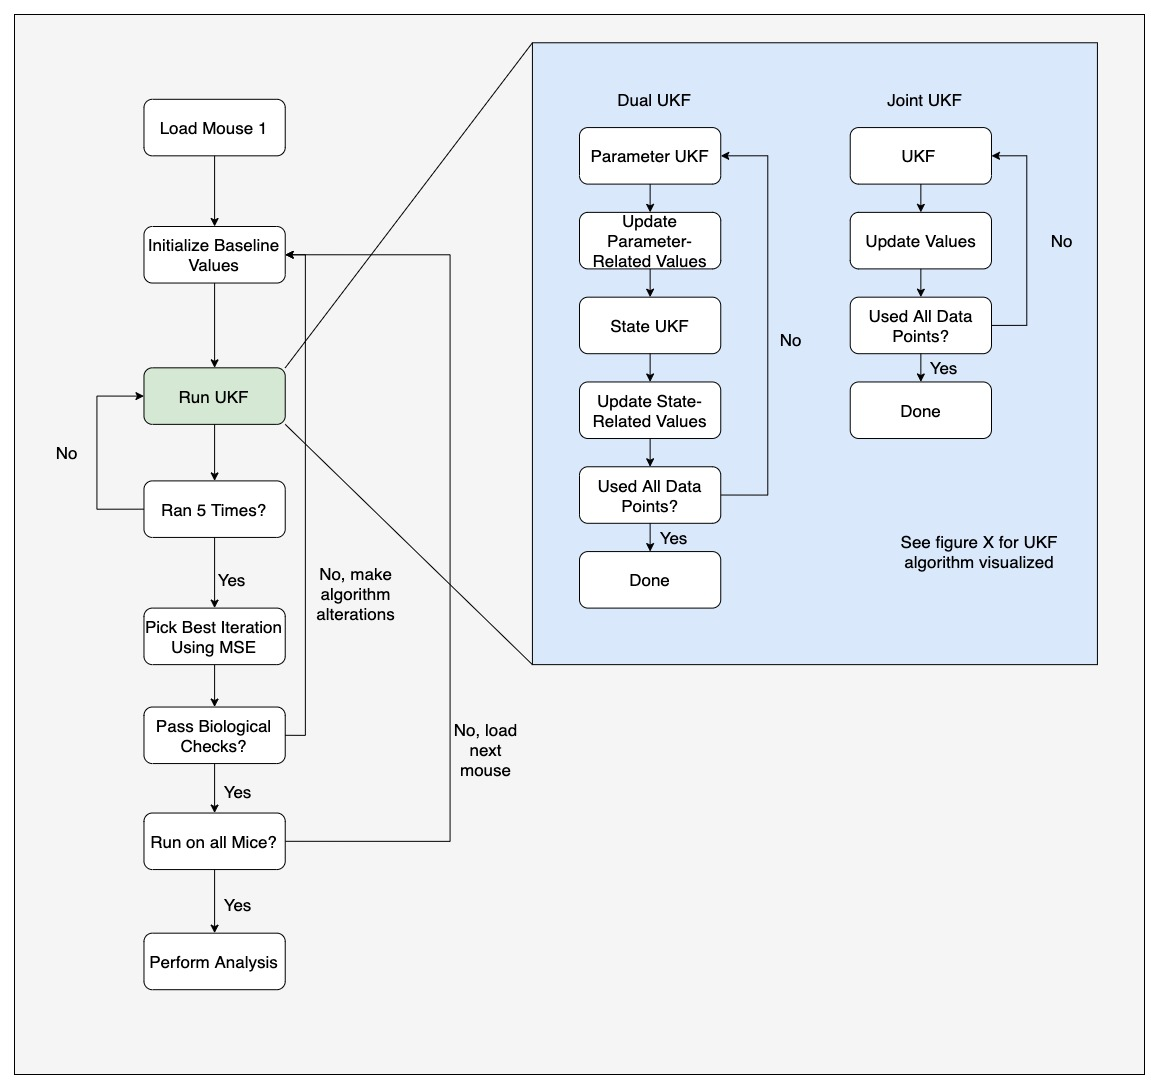
\includegraphics[width=15cm]{Kalman Filter Images/Workflow_FlowChart_Paper.jpg}
    \caption{Flow chart depicting the structure of code used to fit parameters to T1D model. Notice that multiple iterations are performed in order to determine the best fit.}
\end{figure}
In addition to the role of multiple iterations, we can also see here that the general structure of the code is independent of whether a Dual or Joint UKF is being used. Additionally, it demonstrates that Biological Checks as described in 3.2 must be completed before determining that an iteration on a specific mouse has been successful. Lastly, it is important to note that there are occurrances where, for example, the results after iteration 3 are worse than those from iteration 2. This is a surprising result and is why we choose the \emph{best} run of 5 iterations instead of consistently choosing the fifth. This discrepency is likely due to the manner in which parameter variances are set in the algorithm. Towards later iterations the variances are now too high and we should not be searching as much of parameter space as we are. Thus, looking more into how to reduce variances as more and more iterations are completed is recommended.\\
\\
Let us now begin the discussion of the specifics regarding the algorithm set up.




\subsection{Common Parameters}
Once again we begin by considering the values of $\alpha$, $\kappa$, $\beta$, and the measurement noise $R$, values common to the Dual and Joint approaches. $\alpha$ is once again set to a small value, this time 10e-4. Values of $\kappa$ and $\beta$ were kept constant when transitioning to the T1D model from Predator-Prey, meaning that they are 0 and 2 respectively. However, we have a drastic shift in our approach to approximating $R$.\\
\\
Using baseline parameter values from A. Do, we can simulate Glucose values over time. Using this, we can then compare to our measured Glucose values and take the variance of differences at each time point in order to construct $R$. Since we only have a single observable, here $R$ will be a single variance value. Additionally, $R$ can be calculated on a mouse-by-mouse level, helping the algorithm work across a wide range of mice data sets.

\subsection{Dual UKF}
The state space model for the Dual UKF for the T1D model is set up in an analogous way to the predator-prey model. The state space model for the states is set up as a vector of the states represented by the solved version of their respective ODE's  with some process noise added on. The observable equation, which is just glucose, contains a matrix which filters out only glucose from the states, with a little measurement noise added in. \\
\\
The state space model for the parameters is also set up similarly. The state equation for the parameters is a simple identity transformation with a bit of process noise added in. And the observable equation is some function of the parameters that is equal to the value of glucose, with a little bit of measurement noise added in. 

\subsection{Process Covariances}
Let's begin with $Q_x$. In the T1D model, since there is no knowledge of the states apart from Glucose, noise needs to be estimated in an ad hoc fashion. To do this, the feasible range of the state was considered in order to estimate a noise value that was on a similar scale of magnitude to those values. Then, they were tuned in order to better the system's fits. In the end
$$Q_x = diag([10^3 \ 10^3 \ 10^3 \ 700 \ 100 \ 50 \ 2 \ 100 \ 10^3 \ 10^4 \ 100 \ 200])$$
was chosen. Next, follow the same literature used to set $Q_param$ for the Predator-Prey model, meaning that we have
$$ Q_{param} = .01 * P_{param_0} $$ 
here as well.

\subsubsection{Initial State and Parameter Covariances}
Beginning with $P_{x_0}$, we were able to initialize to a square matrix of all ones in the case of T1D. If you recall from Predator-Prey, there covariances between states were left as 0, however here due to the complexity of the interactions between cells in the pancreas it is best to make those non-zero. $P_{params_0}$, as in the Predator-Prey system, proved to be crucial. Eventually, the matrix
$$ P_{params_0} = diag([200 \ 0.05 \ 0.005 \ 0.05 \ 10e-10 \ 10e-10 \ 10e-12 \ 10e-4 \ 10e-3 \ 10 \ 2 \ 2 \ 0.02 \ 5 \ 5$$ 
$$\ 10 \ 175 \ 10^{-3} \ 10^{-3} \ 10^{-3} \ 10^{-3} \ 10^{-3} \ 175 \ 10^{-11} \ 10^{-11} \ 10^{-4} \ 1 \ 4 \ 10^{-3} \ 10^{-5} \ 10^{-5} \ 10^{-5} \ 10^{-3} \ 200 \ 1 \ 1 \ 1 \ 5 \ 15 \ .0001]) $$ %FIX FORMATTING
was decided on. Here, each variance can be traced to its corresponding parameter in the \textbf{Appendix}. In the T1D model, the importance of parameters ranges tremendously. By this we mean that a small shift in some parameters can drastically change the outcome of the system while others are less crucial. Thus, this \emph{sensitivity} is crucial to consider when determining variance values. Additionally, through experimentation, parameters were determined that tended to move from their baseline values more than others. Thus, these values must be assigned larger variances in order to allow for the movement necessary to fit the given data. Specifically, examples of such parameters are found in Table X.\\
\\
Thus, these variances have been determined through experimentation specifically with the Li dataset. In the event that new datasets are incorporated, one will need to consider these variances depending on how similar the data is to the baseline parameter values. Additionally, following new sensitivity analysis results these values will need to be reconsidered as well. 

%POSSIBLY ADD STUFF ABOUT THE SENSITIVITY ANALYSIS

\subsubsection{Dual UKF Results}
We are interested in assessing results on a wide range of mice, including those which are acute as well as progressive. Let's begin with the acute mice.

\paragraph{Acute Mice}
As specified previously, acute mice make a drastic transition from the healthy to unhealthy state, categorized by a "Z" shape in the glucose levels. When the definition is applied to the Li dataset, we are left with 9 data sets. We ran the Dual UKF on each mouse and obtained best fit MSE values by comparing the simulated ODE using the final parameters to the raw dataset. Figure X displays the 9 fits while table Y contains the MSE values.\\

\begin{figure}[H]
    \centering
    \includegraphics[width=15cm]{Kalman Filter Images/All_Mouse_Fits.jpg}
    \caption{All best fits for acute NOD mice. The ODE system using the final parameter estimates is plotted against the raw data. It is evident that the algorithm is functioning correctly, however there is room for improvement, most likely through experimentation with parameter variances.}
\end{figure}

\begin{table}[H]
  \begin{center}
    \label{tab:table1}
    \begin{tabular}{c|c} % <-- Alignments: 1st column left, 2nd middle and 3rd right, with vertical lines in between
      \textbf{Mouse Number} & \textbf{MSE} \\
      \hline
      \textbf{2} & 1.9902e4\\
      \textbf{3} & 4.5462e3\\
      \textbf{4} & 1.6649e3\\
      \textbf{6} & 2.5194e3\\
      \textbf{7} & 4.1531e3\\
      \textbf{8} & 2.5665e3\\
      \textbf{9} & 3.8981e3\\
      \textbf{10} & 2.0596e3\\
      \textbf{11} & 1.3104e4
    \end{tabular}
    \caption{Mean Squared Error (MSE) of ODE simulations using final parameter values for Acute mice from Dual UKF on T1D model. This confirms our visual understanding that errors overall are low however could likely be improved further.}
  \end{center}
\end{table}
It is evident that the Dual UKF is successful across a range of mice, however performance is of course dependent on the data set. Largely, this is due to how "different" that dataset is from the baseline. The baseline parameters produce the glucose values in Figure Z. The more similar the shape of the glucose of a mouse is to that behavior, the better fit we would expect. Thus, in this lies the importance of the initial parameter guess one uses in the algorithm.

\paragraph{Progressive Mice}
In order to examine behavior of Progressive mice, we look at mice 1 and 5. The behavior these mice is a relatively flat glucose slope towards a diabetic state. Our initial hypothesis is that the algorithm will perform poorly on these datasets due to the underlying model being geared more so towards acute behavior. Figure V and Table W once again display the best fit and MSE values.

\begin{figure}[H]
    \centering
    \includegraphics[width=15cm]{Kalman Filter Images/Progressive_Mouse_Fits.jpg}
    \caption{Best fits for the Progressive NOD mice. It is evident that, in general, the algorithm performs worse in this scenario that in the Acute setup. This is most pronounced in Mouse 1.}
\end{figure}

\begin{table}[H]
  \begin{center}
    \label{tab:table1}
    \begin{tabular}{c|c} % <-- Alignments: 1st column left, 2nd middle and 3rd right, with vertical lines in between
      \textbf{Mouse Number} & \textbf{MSE} \\
      \hline
      \textbf{1} & 7.5384e3\\
      \textbf{5} & 7.9402e3
    \end{tabular}
    \caption{Mean Squared Error (MSE) of ODE simulations using final parameter values from Dual UKF run on Progressive mice for the T1D model. Once again, we see the general trend of worse fits on the Progressive, as compared to Acute, mice.}
  \end{center}
\end{table}


As expected, the algorithm performs poorly on the progressive mouse. We can see that, in Mouse 1, the algorithm expects the sudden jump to a diabetic state that we saw in acute mice and thus is tricked by increases in glucose it expects to predict the onset. In fact, it is likely that the algorithm would need to be initiated differently, meaning different covariance matrices and initial guesses, in order to get an ideal fit for a progressive mouse. This is an aspect of the problem that we highly recommend pursuing moving forward.

\subsubsection{Analysis of Parameter Movement}
At the completion of running the Dual UKF, it is helpful to analyze how far away parameters have traveled from their original starting points, as these can be seen as the parameters having the most impact on the outputted fit. In order to gain a general understanding of the important parameters, we can look at the average deviation from the starting point and identify parameters that, on average, move greater than or equal to 0.8\%. For the Dual UKF, those parameters are found in Table X.

\begin{table}[H]
  \begin{center}
    \label{tab:table1}
    \begin{tabular}{c|c} % <-- Alignments: 1st column left, 2nd middle and 3rd right, with vertical lines in between
      \textbf{Parameter} & \textbf{Average Percent Change} \\
      \hline
      \textbf{$e_1$} & 530.965\\
      \textbf{$e_2$} & 1.933e3\\
      \textbf{$\alpha_B$} & 18.215\\
      \textbf{$\delta_B$} & -32.067\\
      \textbf{$S_I$} & 483.671\\
      \textbf{$\sigma_I$} & 1.351\\
      \textbf{$G_I$} & -5.642\\
      \textbf{$\mu$} & 1.353e4\\
      \textbf{$\eta$} & -3.864\\
      \textbf{$EG_0$} & -0.873
    \end{tabular}
    \caption{Parameters and average percent change for all those that exceed 0.8 percent. These parameters appear to be of utmost importance in producing the fits seen in this section.}
  \end{center}
\end{table}

Variances for these parameters in particular were important to tune and it will be crucial to continue delving into their importance moving forward. It will also be interesting to see how these relate to parameters outputted from a formal sensitivity analysis.



\subsection{Joint UKF}

The state space model of the Joint UKF for the T1D model is set up in a similar fashion to the predator-prey model. The latent states are one long vector containing both states and parameters, with the states as solved versions of the equations from the ODE model, and the parameters as themselves, since they are assumed to be constant, with some process noise added. For the observables, the only observable is glucose, which is a state, so the equation for the observables is linear for this system as well. The equation applies a matrix with a 1 in the spot that corresponds to glucose and 0s everywhere else, with some measurement noise added. 

\subsubsection{Process Noise $Q$}
When setting up the process noise matrix ($Q$) for the Joint UKF, we chose to set it up as a block diagonal of the state and parameters process noise matrices from the Dual ($Q_x$ and $Q_{params}$. Thus, the matrix was set as the following:\\
$$Q = \begin{bmatrix} Q_x & 0 \\ 0 & Q_{params} \end{bmatrix}$$

For more information about how these matrices were chosen refer back to the section 3.3.1.

\subsubsection{Initial Covariance $P_0$}
Similarly to the process noise, when setting up the initial covariance matrix ($P_0$) for the Joint UKF, we decided to set it up as a block diagonal of the initial covariance matrices for states and parameters from the Dual ($P_{x_0}$ and $P_{params_0}$, meaning that we had\\
$$P_0 = \begin{bmatrix} P_{x_0} & 0 \\ 0 & P_{params_0} \end{bmatrix}$$\\
For more information on how these matrices were chosen refer back to section 3.3.2. 

\subsection{Treatment of $\eta$ parameter}
One of the most important parameters in the system is the $\eta$ parameter. This can have large effect on the fit, since it has a large effect on the slope of the glucose. While in the Dual, $\eta$ was allowed to vary, in the Joint, letting $\eta$ vary produced worse results. Therefore, it was held constant. However, since it had such a large effect on the system, the fits were run with two different values of $\eta$, 0.01 and 0.018. Changing $\eta$ had large effects on the results for each mouse, which will be discussed further in the results section. 

\subsubsection{Additional Notes on using the Joint UKF with the Li Dataset} - Maybe move this around or different title? Appendix? Specific notes on the code?
When implementing the UKF in matlab, the transition function consists of solving the ODE in between consecutive time points. However, with data sets such as the Li dataset, the differences in time points are not always the same. Therefore, you cannot use a consistent time interval for the ODE solver, but must specify a new one for each iteration. For the Joint UKF, we addressed this by calculating a vector of the different timespans and passing them into the UKF function. 

\subsubsection{Joint UKF Results}

\paragraph{Acute Mice}

\begin{figure}[H]
    \centering
    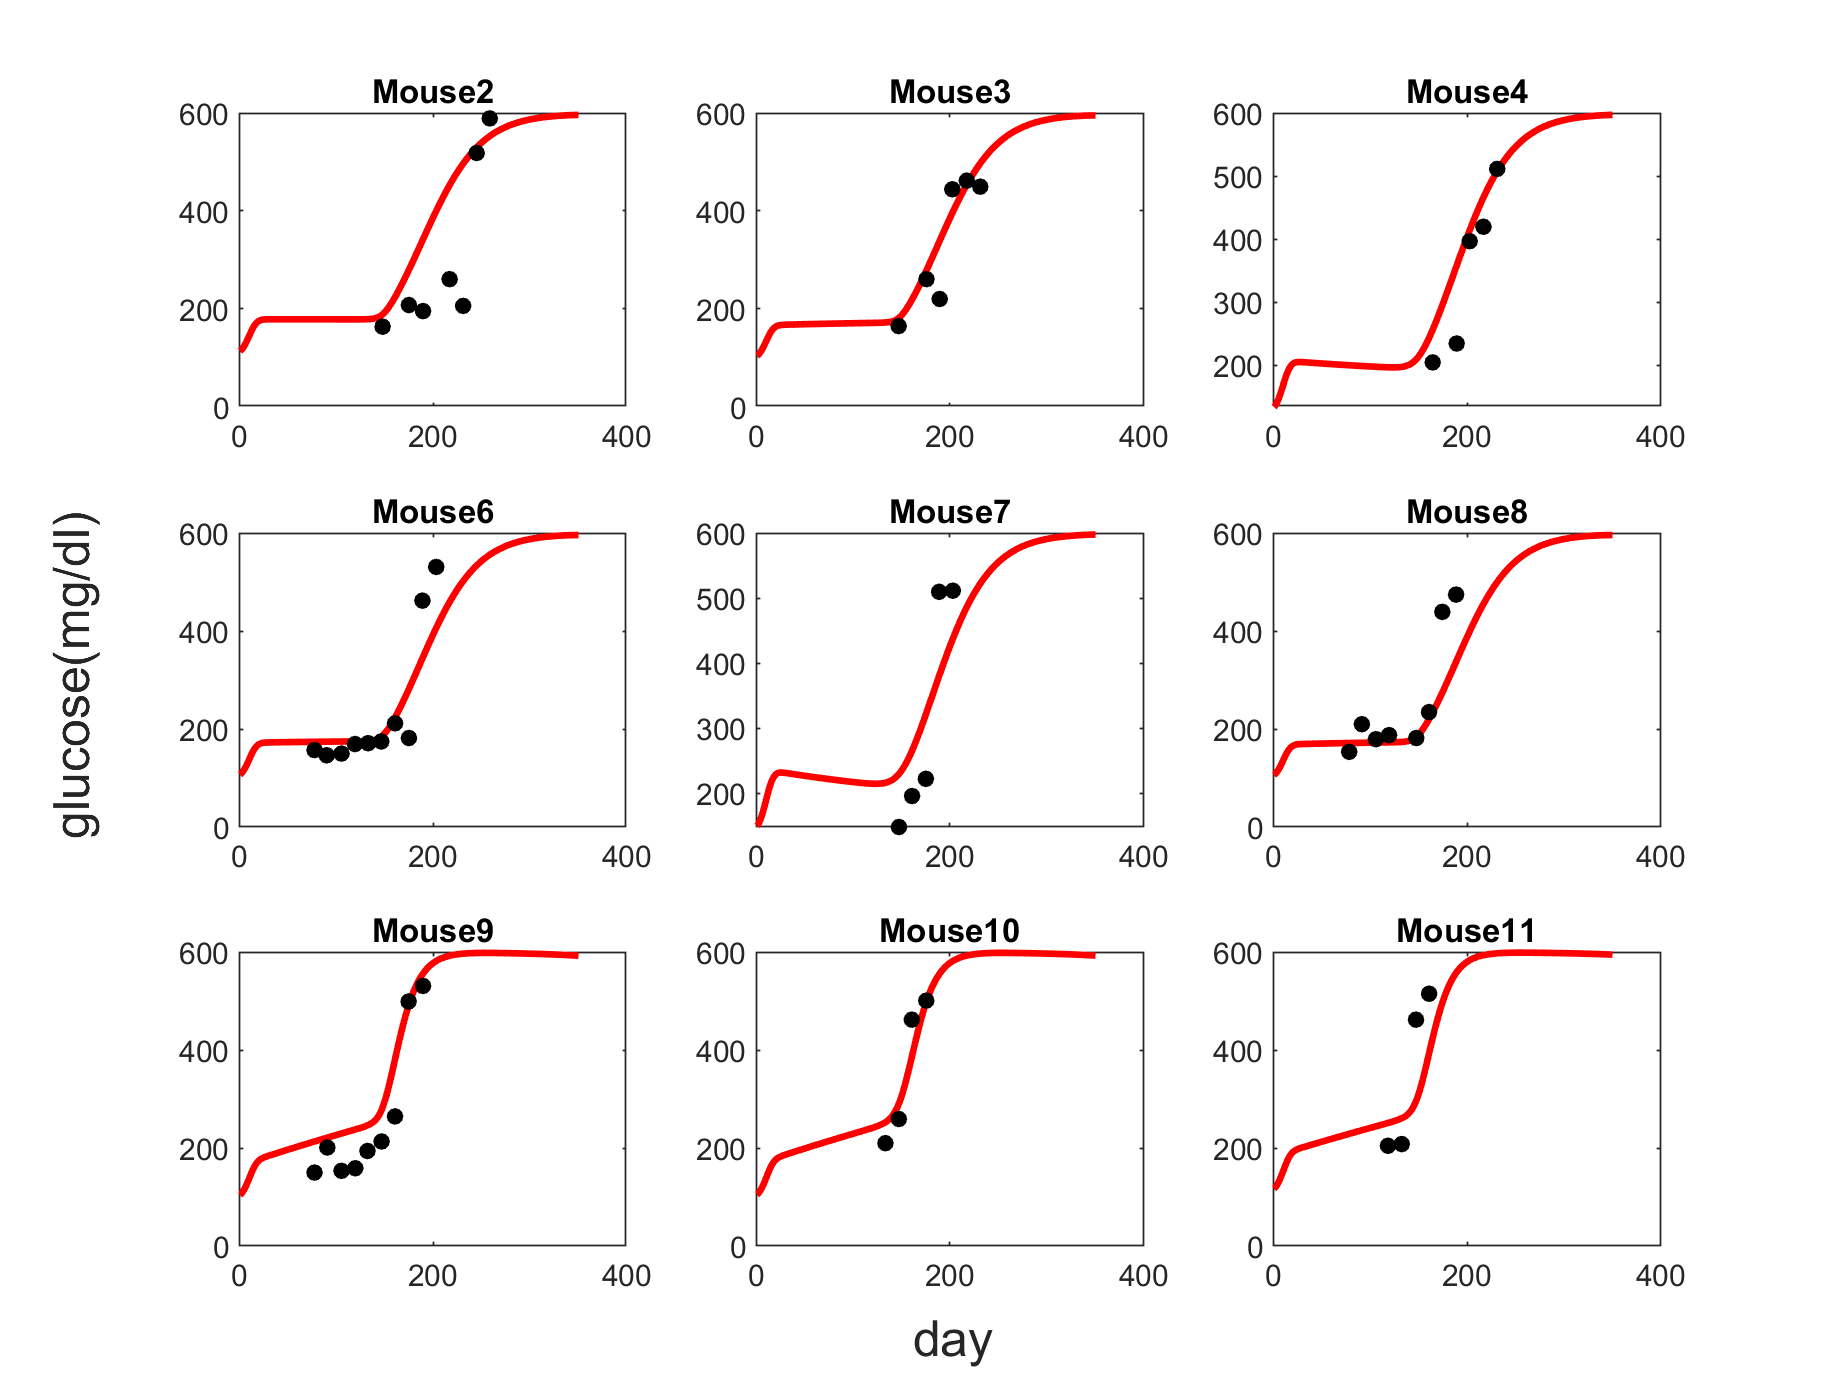
\includegraphics[width=15cm]{Kalman Filter Images/joint_acute_all.png}
    \caption{All best fits for acute NOD mice from the Joint UKF. The ODE system using the final parameter estimates is plotted against the raw data. It is evident that the algorithm is functioning correctly, however there is room for improvement, most likely through experimentation with parameter variances, and possibly with the parameter eta.}
\end{figure}

Below we have the results from the Joint UKF for all of the mice we characterized as acute as well as the mean squared error for each run. We ran the filters on the mice for two different eta values, 0.01 and 0.018. Mice 1-9 had far better results with an eta value of  0.01 and mice 9-11 had far better results  with an eta value of 0.018. In each case, the resulting differences were quite significant, reducing the MSE between 33 and 78 percent. The fits above show the best results.

\begin{table}[H]
  \begin{center}
    \label{tab:table1}
    \begin{tabular}{c|c} % <-- Alignments: 1st column left, 2nd middle and 3rd right, with vertical lines in between
      \textbf{Mouse Number} & \textbf{MSE} \\
      \hline
      \textbf{2} &  2.6312e4\\
      \textbf{3} & 3.3472e4\\
      \textbf{4} & 2.6113e3\\
      \textbf{6} & 4.5054e3\\
      \textbf{7} & 8.9870e3\\
      \textbf{8} & 4.1695e3\\
      \textbf{9} & 4.3284e3\\
      \textbf{10} & 2.1669e3\\
      \textbf{11} & 1.2078e4
    \end{tabular}
    \caption{Mean Squared Error (MSE) of ODE simulations using final parameter values for Acute mice from Joint UKF on T1D model. This confirms our visual understanding that the errors are low although in many cases further improvement is possible.}
  \end{center}
\end{table}

The Joint UKF is successful in creating relatively good fits. However, it seems that a lot of the fit is dependent on the value of eta and that the optimal value of eta is likely different for each mouse, since mice 1-8 performed substantially better with an eta value of 0.01 and mice 9-11 performed substantially better with an eta value of 0.018. This is definitely something that could be explored in the future. When eta was allowed to vary in the past, the results were not improved, however, it might be worth trying again on different mice or with a different variance or starting value. Additionally, even it is decided that eta is better off constant, it could be valuable to tune  eta specifically to each mouse, possibly by running the algorithm multiple times with different values of eta.

\paragraph{Progressive Mice}

\begin{figure}[H]
    \centering
    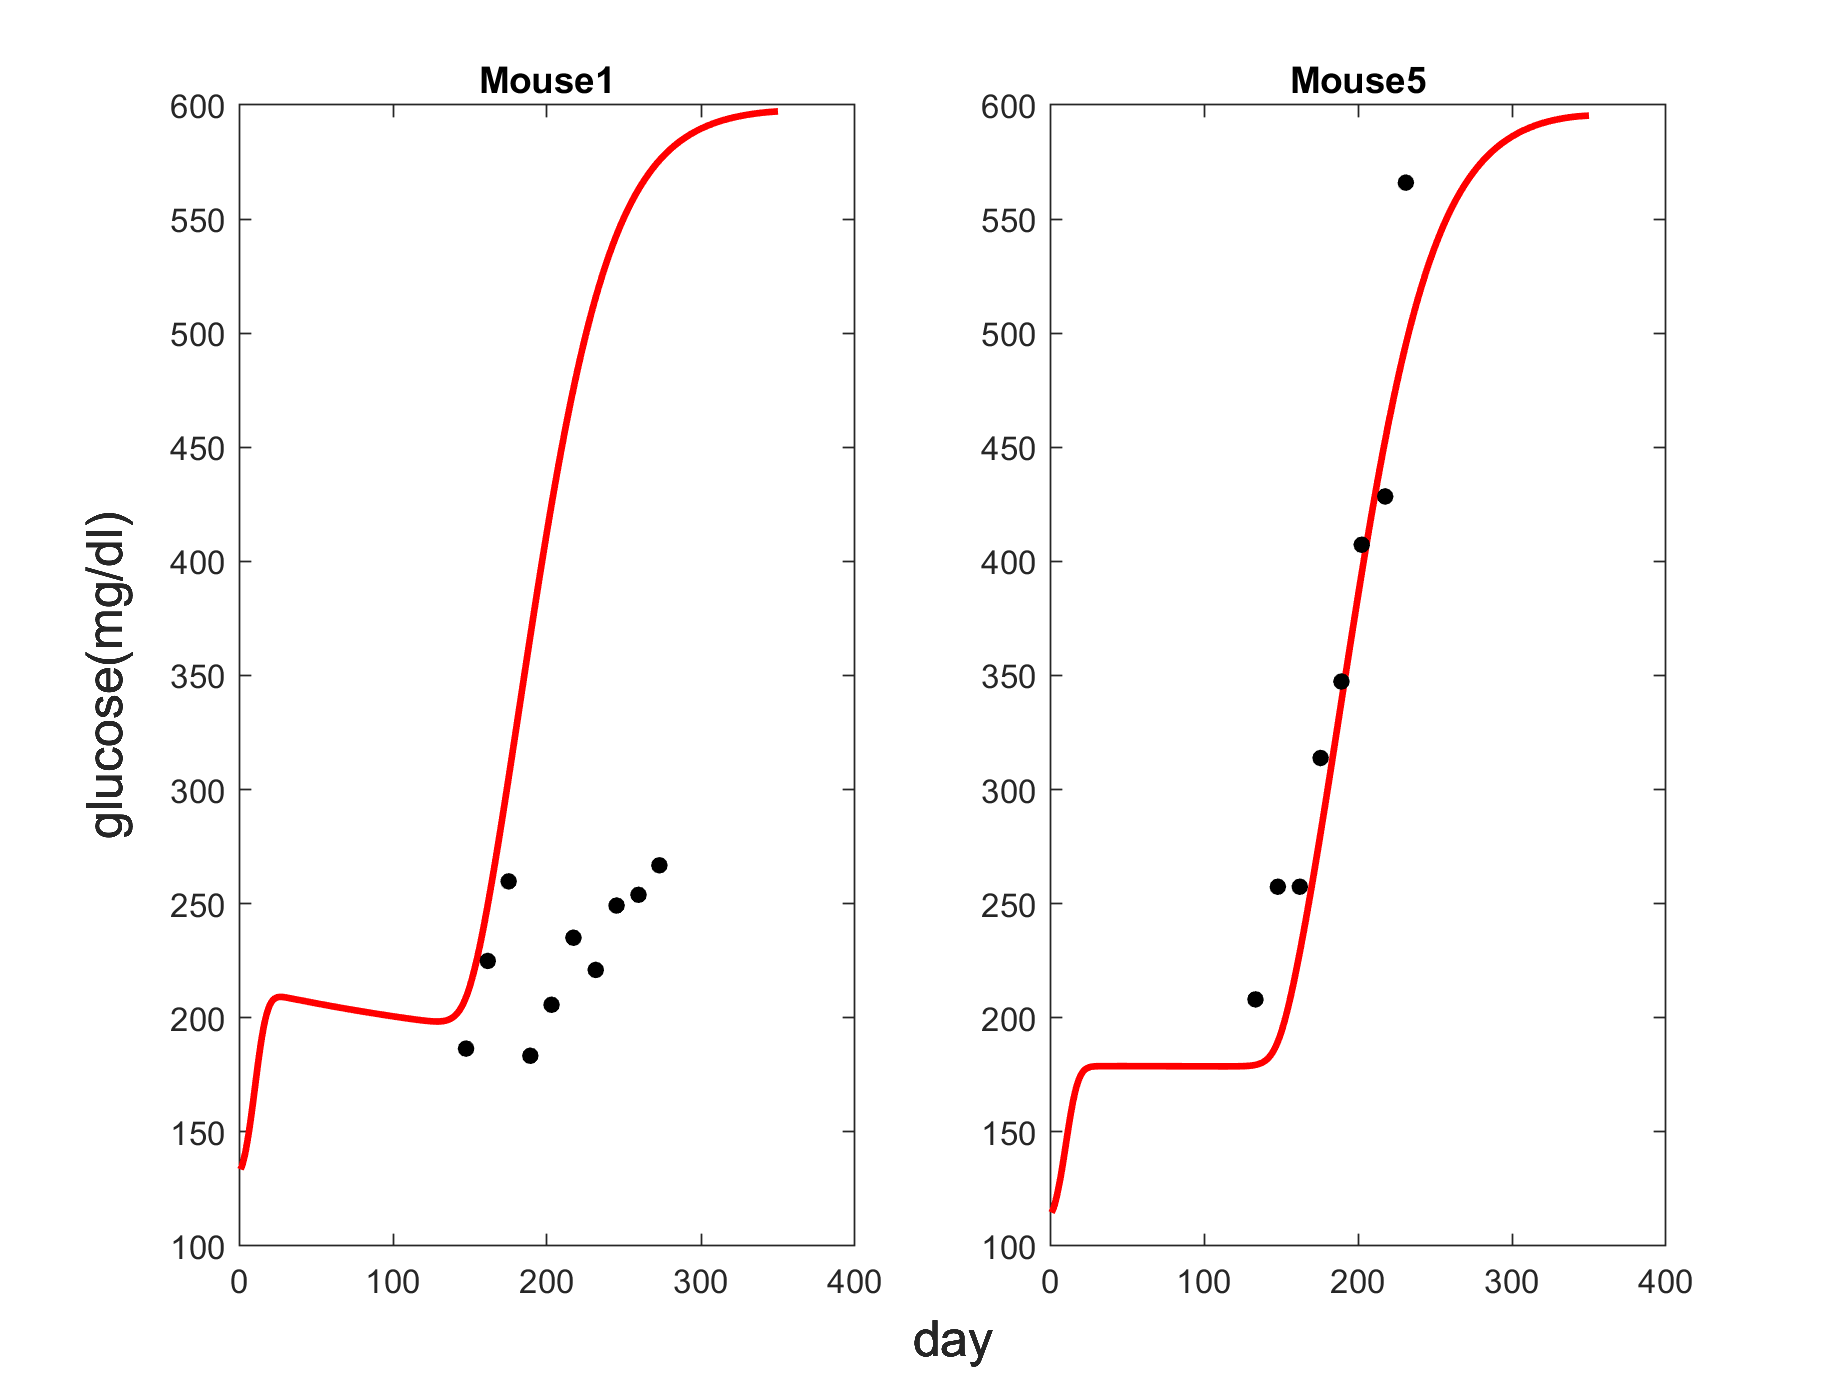
\includegraphics[width=15cm]{Kalman Filter Images/joint_progressive_all.png}
    \caption{Best fits for the Progressive NOD mice. It is evident that, in general, the algorithm performs worse in this scenario that in the Acute setup. This is most pronounced in Mouse 1.}
\end{figure}

\begin{table}[H]
  \begin{center}
    \label{tab:table1}
    \begin{tabular}{c|c} % <-- Alignments: 1st column left, 2nd middle and 3rd right, with vertical lines in between
      \textbf{Mouse Number} & \textbf{MSE} \\
      \hline
      \textbf{1} & 4.3713e4\\
      \textbf{5} & 974.6495
    \end{tabular}
    \caption{Mean Squared Error (MSE) of ODE simulations using final parameter values from Joint UKF run on Progressive mice for the T1D model. We see a much worse fit for Mouse 1, however we see an excellent fit for Mouse 5.}
  \end{center}
\end{table}

Unlike the Dual, while the algorithm performs worse on Mouse 1, the algorithm performs exceedingly well on Mouse 5. This makes sense because while Mouse 5 does not have the sharp spike of the other mice, it still follows the general shape of the model relatively closely  and eventually reaches close to the same point, while Mouse 1 has a very flat slope that does not match the model at all, and never reaches the high levels of glucose that the other mice reach within this timeframe. 

\subsubsection{Analysis of Parameter Movement}

Once again, we are interested in how much parameter movement is going on during the process of running the UKF.
Using the 0.8\% difference threshold once again, we identify the parameters in Table X.


\begin{table}[H]
  \begin{center}
    \label{tab:table1}
    \begin{tabular}{c|c} % <-- Alignments: 1st column left, 2nd middle and 3rd right, with vertical lines in between
      \textbf{Parameter} & \textbf{Average Percent Change} \\
      \hline
      \textbf{$e_1$} & -1.2536\\
      \textbf{$e_2$} & -19.2044\\
      \textbf{$S_I$} & 14.1834\\
      \textbf{$G_I$} & -11.2054\\
      \textbf{$\mu$} & -9,4841\\
      \textbf{$\alpha_{eta}$} & 12.0008\\
    \end{tabular}
    \caption{Parameters and average percent change for all those that exceed and absolute value of 0.8\%. These parameters appear to be of utmost importance in producing the fits seen in this section. Many of the other parameters did not change at all or decreased extremely small amount, much smaller than 0/8\%.}
  \end{center}
\end{table}

One interesting difference to note between the Dual and the Joint is that some of the parameters that tend to increase in the Dual decrease in the Joint instead. Additionally, the number of critical parameters seen here is less than those in Table X (the dual table). This is due to the general trend we have experienced with working with the Joint UKF on the T1D model that parameters tend to experience less movement than in the Dual.


\subsection{Comparison of Dual and Joint UKF Results}

\subsubsection{Biological Checks}
For the purpose of the biological checks we will be focusing on \emph{acute} mice due to the relative success we have had in terms of glucose fits on those mice. Additionally, \emph{mouse 6} will be used as the standard throughout this section, although the general trends of these results are the same across the 9 acute data sets. The first biological check is to plot the 11 states (all except glucose) as simulated for an NOD mouse with an apoptotic wave and using the final parameter values for mouse 6 as shown in figure X. Additionally, we compare this to the system as simulated with the baseline parameter values, which are known to be biologically plausible. We will plot our results from both the Dual\and the Joint UKFs. \\

NOTE: THIS FIGURE IS SUPER FUZZY AND UNREADABLE SO NEED TO FIX

\begin{figure}[H]
    \centering
    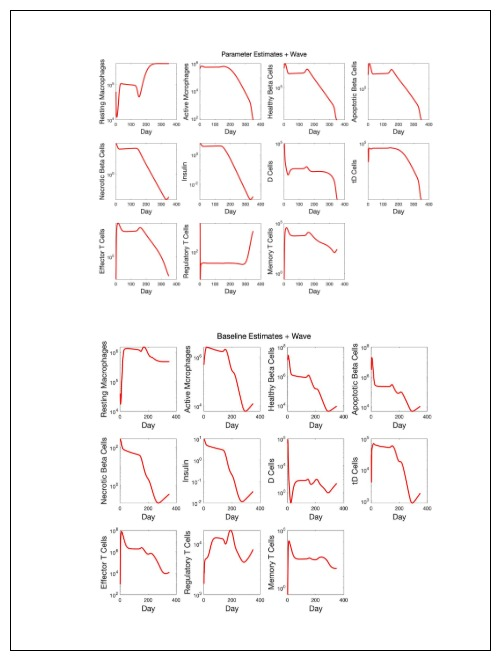
\includegraphics[width=15cm]{Kalman Filter Images/DualStates_WithWave_FullFigure.jpg}
    \caption{Immune cell states simluated using baseline parameters, which are known to produce biologically plausible results (bottom) and with final estimates from Dual UKF on mouse 6 (top). It is evident that the predicted states may be plausible, however do differ in behavior and appear smoother than those produced by the baseline}

\end{figure}

\begin{figure}[H]
    \centering
    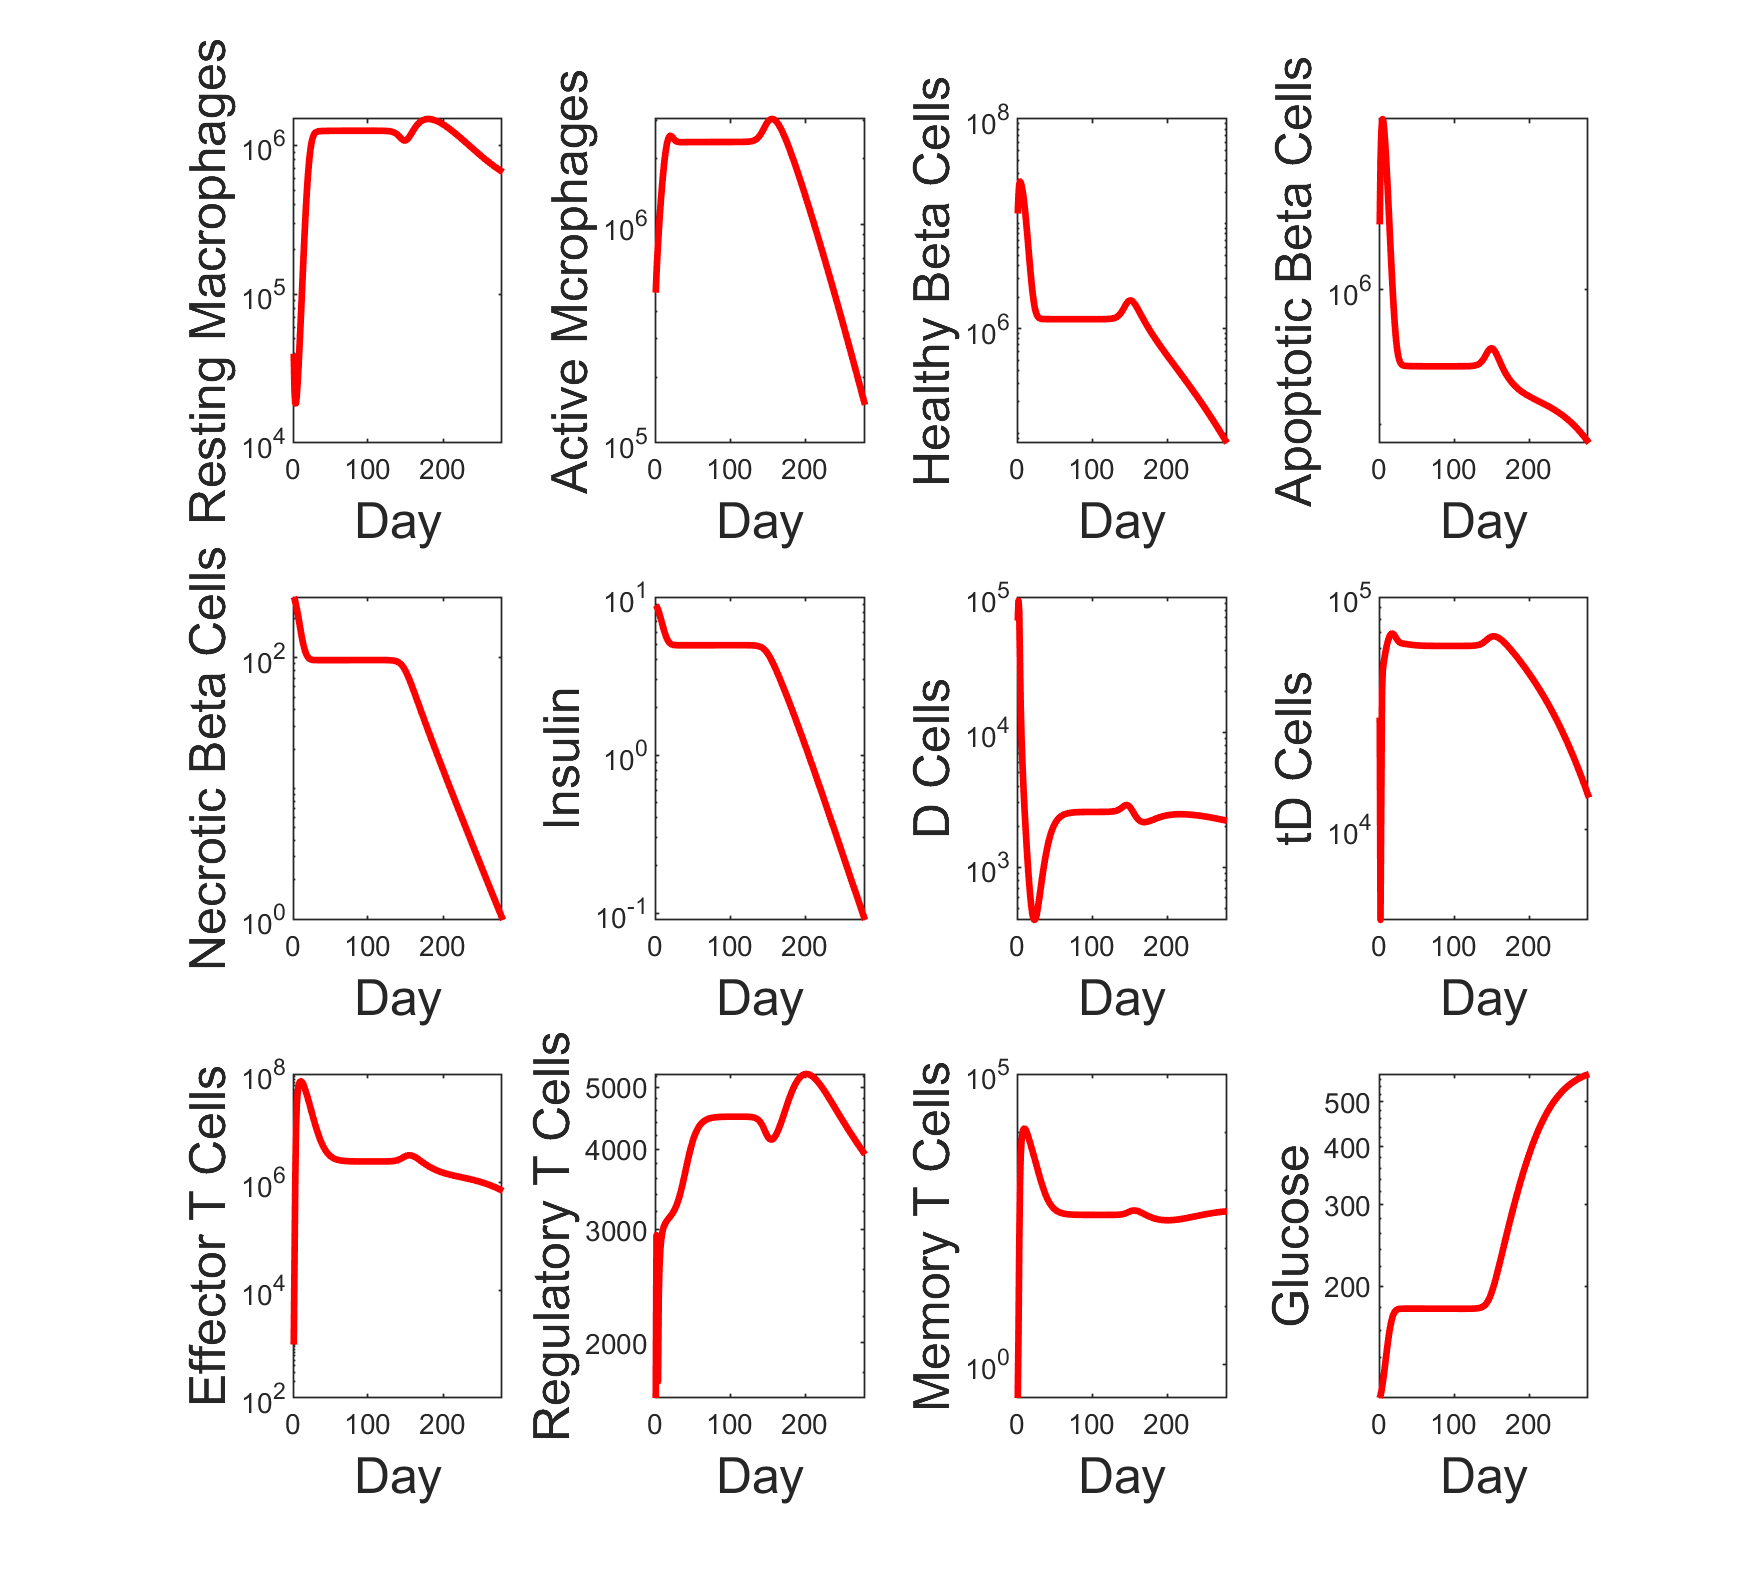
\includegraphics[width=15cm]{Kalman Filter Images/mouse6stateswave.png}
    \caption{Immune cell states simluated the Joint UKF on mouse 6. While most of the states seem to be smmother than the baseline predictions, the overall shapes match up well.}

\end{figure}

First off, it is assuring to see that none of our predicted states do anything extremely outlandish. The main difference we see is in the Regulatory T Cells. With baseline parameters the Regulatory T Cells follow more of a curved path, while under our estimates they flat line relatively early. A main parameter that controls the Regulatory, as well as Effector, is their rates of interaction $\mu_e$ and $\mu_r$. In simplest terms, these control how good each type of T cell is at killing off the other. In the current set up, these are two separate parameters. However, in the baseline they are set to be equivalent. One idea we tried was thus to treat them as a single parameter in our UKF, however this unfortunately, and surprisingly, resulted in nearly identical results. Thus, T cell behavior continues to be one of the aspects needed to be explored further. Of course, there is a possibility that the results from the parameter estimate are actually feasible, however this could not be confirmed without raw T cell data. Additionally, the results from the final parameter estimates produce much smoother curves. This, most likely, is inaccurate and must be explored further as well.\\
%add comparison between dual and joint?
\\
A second biological check is done by producing a figure with final parameters on an NOD mouse with no wave. Here we would expect for the mouse to return to a healthy state, which can be determined by looking at the predicted Glucose plot, which we will now include in our figure, specifically figure Y.\\

\begin{figure}[H]
    \centering
    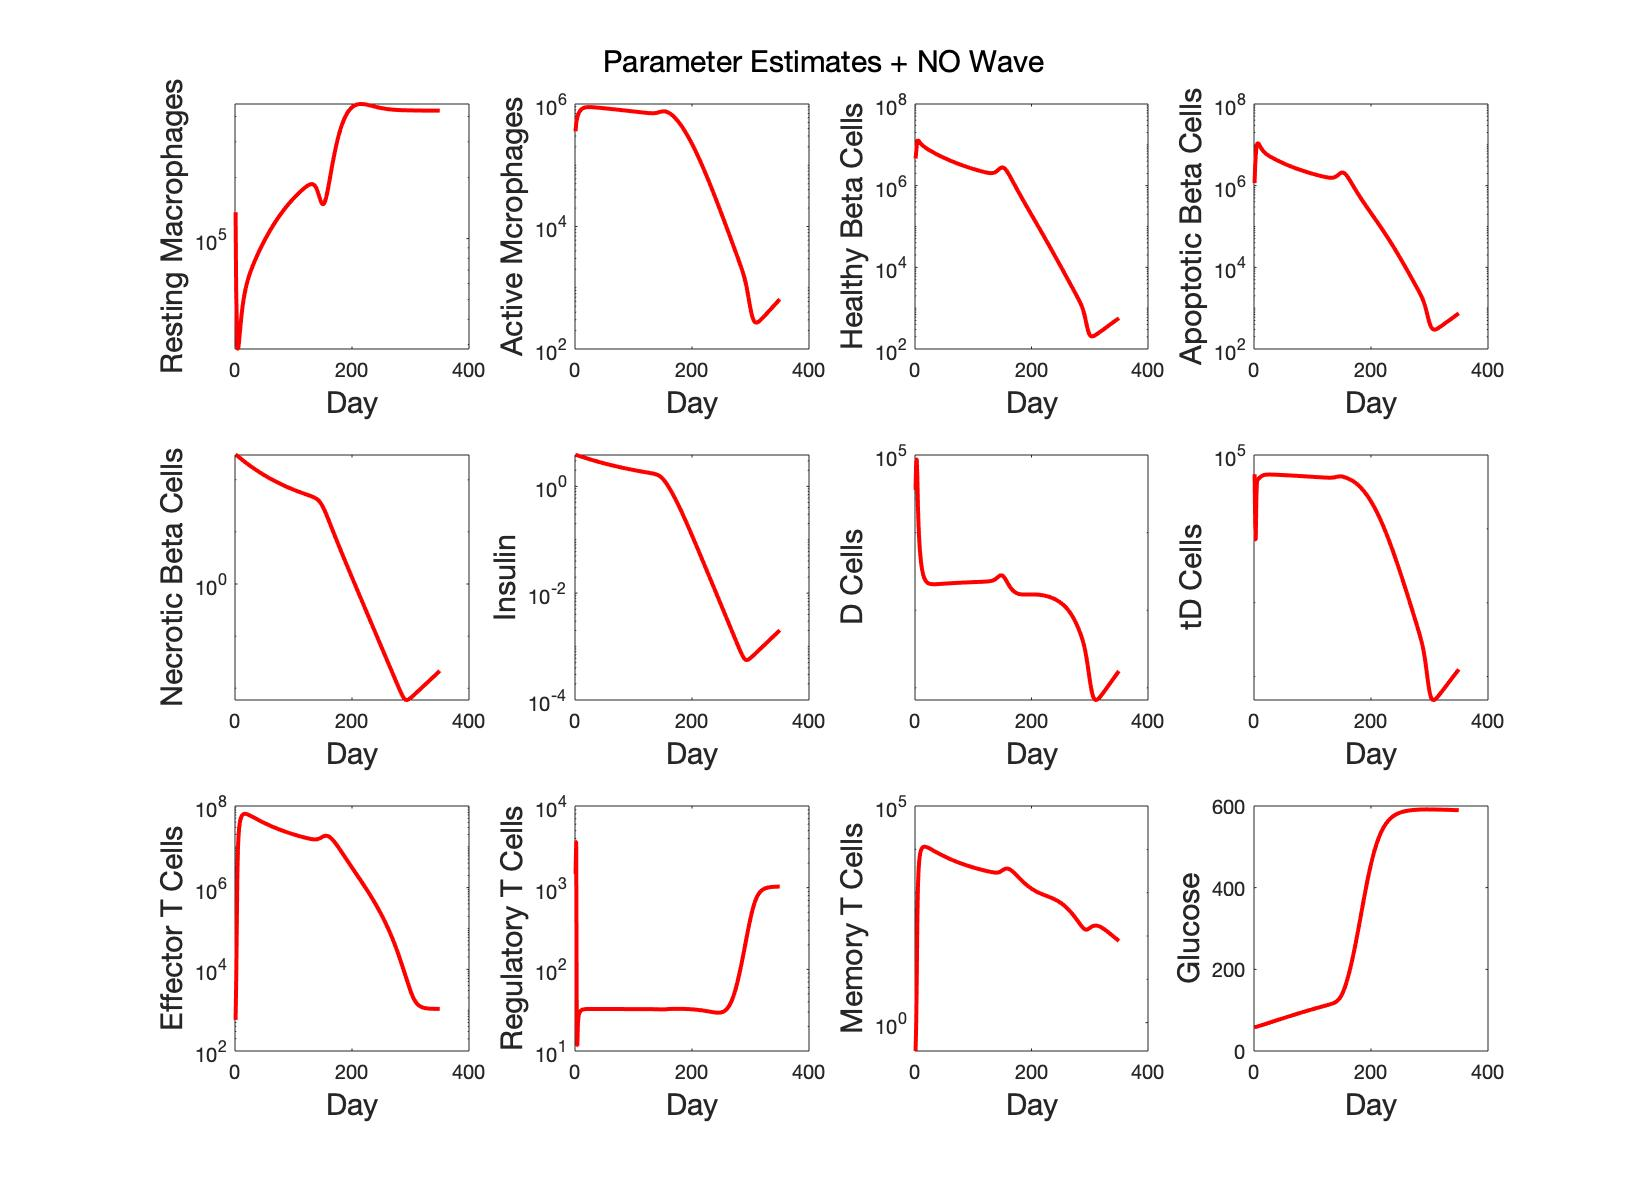
\includegraphics[width=15cm]{Kalman Filter Images/FINAL_DualNoWaveStates.jpg}
    \caption{Immune cell states (including Glucose) simulated using final parameters for mouse 6 when no apoptotic wave present. We are most interested in the panel depicting Glucose to see that the mouse still reaches the unhealthy state.}

\end{figure}



\begin{figure}[H]
    \centering
    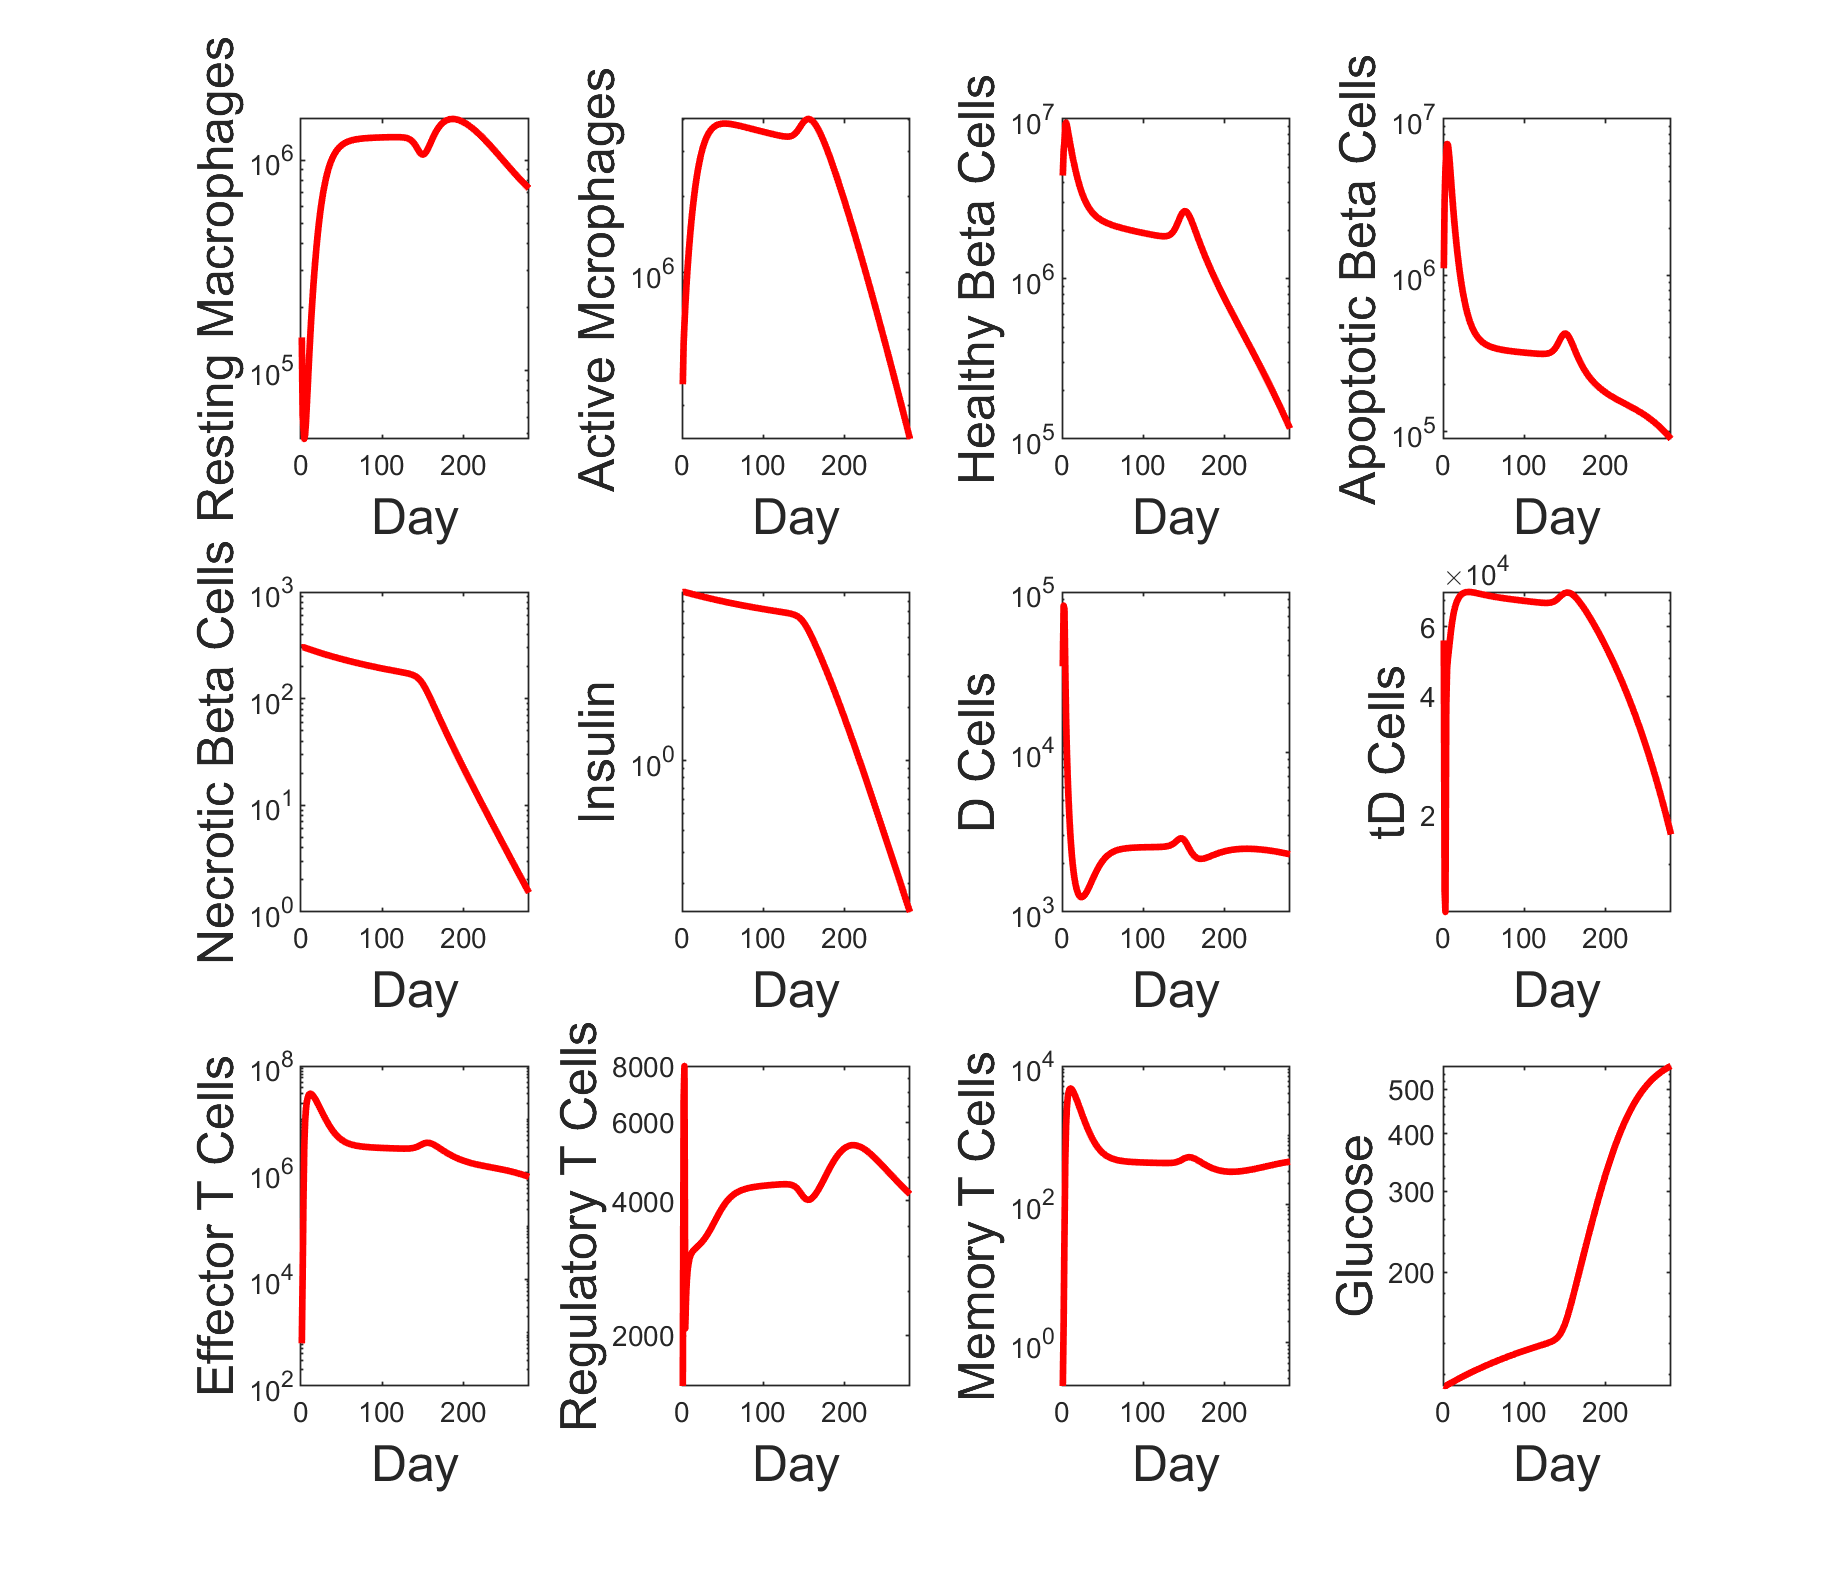
\includegraphics[width=15cm]{Kalman Filter Images/mouse6statesnowave.png}
    \caption{Immune cell states (including Glucose) simulated using final parameters from the Joint UKF for mouse 6 when no apoptotic wave present. We see that unlike the baseline, the mouse still reaches a diabetic state. This is something we would hope to rectify in further research.}

\end{figure}


Looking at the bottom right panel, the glucose estimates, we unfortunately see that, both for the Joint and Dual UKF's, our mouse is still getting sick, even though no wave is present. Our current best guess is that this is due to the relationship between $\eta$ and the macrophage clearance rates. When developing the baseline parameters, these were found to be extremely sensitive and, in the process of parametrization, it is likely that the relationship between them all is becoming distorted. Specifically, $\eta$ is currently one of the parameters being estimated while the clearance rates are one of the few being held constant because of their extreme sensitivity. However, if $\eta$ continues to be estimated, a decision will need to be made on how to move the clearance rates to more biologically acceptable values.

\section{Overview}
Here we have described the general process one follows to implement, and have displayed the results following such a process, the Joint and Dual Unscented Kalman Filters on two biological systems of varying complexities. In general, we have been more impressed by the performance of the UKF algorithms on the more complex T1D model, which is initially surprising. However, this exposes the importance of the underlying model that is used to capture the system. For example, the Lotka-Volterra systems reliance on only 4 parameters limits the goodness of fit one can obtain to a noisy set of data, which is not the case in the T1D set up. Due to the UKF's reliance on the underlying model, particularly in the \emph{Update Step} via the Transition Matrix $F_{k,k-1}$, one should pay a great deal of attention to the model they are using before implementing a UKF. Additionally, when analyzing results it is important to have an understanding of the limits the model sets on how close a fit one is capable of obtaining.\\
\\
A second important conclusion we draw from our experimentation is a preference for the Dual UKF as compared to the Joint. In both the Lotka-Volterra and T1D systems, the ability of the Dual to separate out noise and covariances between states and parameters has proven to be more important than the covariance between state and parameters introduced by the Joint. Thus, moving forward on the T1D model, our recommendation is to focus on the Dual UKF as the parametrization algorithm.